\begin{name}
	{\tenchude}
	{TOÁN 11}
	{LỚP TOÁN THẦY PHÁT}
	{Thời gian: 90 phút - Không kể thời gian phát đề}
\end{name}
\setcounter{ex}{0}\setcounter{bt}{0}
\TN
\Opensolutionfile{ans}[ans/ansDe1-TN1]
\begin{ex}%[1H8N1-1]
	Mệnh đề nào sau đây là \textbf{đúng}?
	\choice
	{Hai đường thẳng cùng vuông góc với một đường thẳng thì song song với nhau}
	{Một đường thẳng vuông góc với một trong hai đường thẳng vuông góc với nhau thì song song với đường thẳng còn lại}
	{\True Một đường thẳng vuông góc với một trong hai đường thẳng song song thì vuông góc với đường thẳng còn lại}
	{Hai đường thẳng cùng vuông góc với một đường thẳng thì vuông góc với nhau}
	\loigiai{
		\begin{itemize}
			\item \lq\lq  Hai đường thẳng cùng vuông góc với một đường thẳng thì song song với nhau\rq\rq  là mệnh đề \textbf{sai} vì hai đường thẳng đó có thể cắt hoặc chéo nhau.
			\item \lq\lq  Một đường thẳng vuông góc với một trong hai đường thẳng vuông góc với nhau thì song song với đường thẳng còn lại\rq\rq  là mệnh đề \textbf{sai} vì hai đường thẳng đó có thể cắt hoặc chéo nhau.
			\item \lq\lq  Một đường thẳng vuông góc với một trong hai đường thẳng song song thì vuông góc với đường thẳng còn lại\rq\rq  là mệnh đề \textbf{đúng}.
			\item \lq\lq  Hai đường thẳng cùng vuông góc với một đường thẳng thì vuông góc với nhau\rq\rq  là mệnh đề \textbf{sai}.
		\end{itemize}}
\end{ex}

\begin{ex}%[1H8H2-2]
	\immini{Cho hình chóp $S. ABCD$ có $SA\perp AB$, $SA\perp AC$. Khẳng định nào dưới đây đúng?
		\choice
		{$SA\perp(SBC)$}
		{$SA\perp(SCD)$}
		{\True $SA\perp(ABCD)$}
		{$SA\perp(SAB)$}}
	{
		\begin{tikzpicture}[scale=1,>=stealth, font=\footnotesize, line join=round, line cap=round,declare function={h=2.5;}]
			\path
			(0,0) coordinate (A)
			(-1.3,-1) coordinate (B)
			(2.5,-1) coordinate (C)
			(barycentric cs:A=1,C=1,B=-1)coordinate(D)
			(A)+(90:h) coordinate (S)
			;
			\draw[dashed] (S)--(A)--(B)--(D)  (C)--(A)--(D);
			\draw (C)--(S)--(B)--(C)--(D)--(S);
			\pic[draw,angle radius=5]{right angle=S--A--B};
			\pic[draw,angle radius=5]{right angle=S--A--C};
			\foreach \p/\g in{A/-85,B/-90,C/-90,D/-45,S/90}
			\fill[black](\p)circle(.03)node[shift={(\g:.25)},scale=1]{$\p$};
		\end{tikzpicture}
	}
	\loigiai{
		Vì $SA\perp AB$, $SA\perp AC$ nên $SA\perp(ABCD)$.
	}
\end{ex}

\begin{ex}%[1H8N6-2]%[Dự án đề kiểm tra Toán 11 HK2 NH23-24- Nguyễn Hữu Duy]%[THPT Chuyên Hùng vương - Phú Thọ]
	\immini{
		Cho hình chóp $S.ABCD$ có đáy $ABCD$ là hình vuông tâm $O$, cạnh bên $SA$ vuông góc với mặt phẳng đáy (tham khảo hình vẽ bên). Khi đó một góc phẳng của góc nhị diện $[S,BD,C]$ là
		\choice
		{$\widehat{SCA}$}
		{$\widehat{SOD}$}
		{$\widehat{SOA}$}
		{\True $\widehat{SOC}$}
	}{
		\begin{tikzpicture}[scale=0.7, font=\footnotesize,line join=round, line cap=round, >=stealth]
			\path
			(0,0) coordinate (A)
			++(-140:3) coordinate (B)
			++(0:4.5) coordinate (C)
			($(A)+(C)-(B)$) coordinate (D)
			($(A)+(0,4)$) coordinate (S)
			($(A)!1/2!(C)$) coordinate (O)
			;
			\foreach \i in{B,C,D}{\draw (S)--(\i);};
			\draw (B)--(C)--(D);
			\draw[dashed] (O)--(S)--(A)--(B) (C)--(A)--(D)--(B);
			\pic[draw,angle eccentricity=1.8,angle radius=2mm]{right angle=S--A--D};
			\foreach \i/\g in {A/180,B/-120,C/-60,D/-60,S/90,O/-90}
			\fill[black] (\i) circle(1pt)+(\g:3mm)node[scale=1]{$\i$};
		\end{tikzpicture}
	}
	\loigiai{
		\immini{Vì $AC \perp BD$, $SA \perp BD$ nên $BD \perp (SAC)$. Vậy $AC$ và $SO$ vuông góc với $BD$. Suy ra $\widehat{SOC}$ là một góc phẳng của góc nhị diện $[S,BD,C]$.
		}
		{
			\begin{tikzpicture}[scale=0.7, font=\footnotesize,line join=round, line cap=round, >=stealth]
				\path
				(0,0) coordinate (A)
				++(-140:3) coordinate (B)
				++(0:4.5) coordinate (C)
				($(A)+(C)-(B)$) coordinate (D)
				($(A)+(0,4)$) coordinate (S)
				($(A)!1/2!(C)$) coordinate (O)
				;
				\foreach \i in{B,C,D}{\draw (S)--(\i);};
				\draw (B)--(C)--(D);
				\draw[dashed] (O)--(S)--(A)--(B) (C)--(A)--(D)--(B);
				\pic[draw,angle eccentricity=1.8,angle radius=2mm]{right angle=S--A--D};
				\foreach \i/\g in {A/180,B/-120,C/-60,D/-60,S/90,O/-90}
				\fill[black] (\i) circle(1pt)+(\g:3mm)node[scale=1]{$\i$};
			\end{tikzpicture}}
	}
\end{ex}

\begin{ex}%[1D6N2-2]
	Với $ a$ là số thực dương tùy ý, $\log_2\left(\dfrac{64}{a^4}\right)$ bằng
	\choice
	{\True $ 6-4\log_2a$}
	{$ 6+4\log_2a$}
	{$ 5+4\log_2a$}
	{$ 6+\dfrac{1}{4}\log_2a$}
	\loigiai{
		Ta có $\log_2\left(\dfrac{64}{a^4}\right)=\log_264-\log_2a^4=6-4\log_2a$.}
\end{ex}

\begin{ex}%[1H8H6-2]
	Cho hình chóp $S. A B C$ có $S A \perp(A B C)$, $A B \perp B C$, $S A=A B=3 a$, $B C=4 a$. Gọi $\alpha$ là số đo của các góc nhị diện $[B, S A, C]$. Tính $\cos \alpha$.
	\choice
	{$\cos \alpha=\dfrac{1}{2}$}
	{\True $\cos \alpha=\dfrac{3}{5}$}
	{$\cos \alpha=\dfrac{1}{5}$}
	{$\cos \alpha=\dfrac{\sqrt{2}}{5}$}
	\loigiai{
		\immini{
			Vì $S A \perp(A B C)$, $A B \subset(A B C)$, $A C \subset(A B C)$\\
			nên $S A \perp A B$, $S A \perp A C$. Suy ra góc $B A C$ là góc phẳng nhị diện của $[B, S A, C]$, hay $\widehat{B A C}=\alpha$. Xét tam giác $A B C$ vuông tại $B$ có
			\[A C=\sqrt{A B^2+B C^2}=\sqrt{(3 a)^2+(4 a)^2}=5 a. \]
			và $\cos \alpha=\cos \widehat{B A C}=\dfrac{B A}{A C}=\dfrac{3 a}{5 a}=\dfrac{3}{5}$.

		}{
			\begin{tikzpicture}[>=stealth,line join=round,line cap=round,font=\footnotesize,scale=0.7]
				\def\a{5};
				\def\b{2};
				\def\g{-40};
				\def\cao{4};
				\path
				(0,0) coordinate (A)
				(0:\a) coordinate (C)
				(\g:\b) coordinate (B)
				($(A)+(90:\cao)$) coordinate (S)
				($(S)!0.4!(B)$) coordinate (H)
				($(S)!0.6!(C)$) coordinate (K)
				;
				\draw (S)--(A)--(B)--(C)--(S)--(B);
				\draw[dashed] (A)--(C) ;
				\foreach \x/\g in {A/180,B/-90,C/0,S/90}\fill[black](\x) circle (1pt) +(\g:3mm) node {$\x$};
				\pic[draw,angle radius=2mm]{right angle=A--B--C};
			\end{tikzpicture}
		}
	}
\end{ex}

\begin{ex}%[Dự án BG K10, K11, Đợt 4]%[Võ Hoàng Nghĩa, Năm học 2024 2025]%[1H8N4-1]
	Khẳng định nào sau đây là đúng?
	\choice
	{$\heva{&\left(\alpha\right)\ne\left(\beta\right)\\&\left(\alpha\right)\perp (P)\\&\left(\beta\right)\perp (P)}
			\Rightarrow \left(\alpha\right)\parallel\left(\beta\right)$}
	{\True $\heva{&\left(\alpha\right)\parallel\left(\beta\right)\\&(P)\perp \left(\alpha\right)}
			\Rightarrow (P)\perp \left(\beta\right)$}
	{$\heva{&\left(\alpha\right)\perp \left(\beta\right)\\&a\subset\left(\alpha\right)\\&b\subset\left(\beta\right)}\Rightarrow a\perp b$}
	{$\heva{&\left(\alpha\right)\perp \left(\beta\right)\\&a\subset\left(\alpha\right)}\Rightarrow a\perp \left(\beta\right)$}
	\loigiai{
		Một mặt phẳng vuông góc với một trong hai mặt phẳng song song thì sẽ vuông góc với mặt phẳng còn lại.
	}
\end{ex}

\begin{ex}%[1D6N1-2]%[Dự án đề kiểm tra Toán 11 HK II NH23-24 - Nguyễn Thành Sơn]%[THPT Nguyễn Thái Bình - Tp.HCM]
	Cho $x$, $y$ là hai số thực dương và $m$, $n$ là hai số thực tùy ý. Đẳng thức nào sau đây là \textbf{sai}?
	\choice
	{$x^m \cdot x^n=x^{m+n}$}
	{$\left(x^n\right)^m=x^{n m}$}
	{\True $x^m \cdot y^n=(x y)^{m+n}$}
	{$(x y)^n=x^n \cdot y^n$}
	\loigiai{
		Đẳng thức $x^m \cdot y^n=(xy)^{m+n}$ \textbf{sai}.
	}
\end{ex}

\begin{ex}%[BG - 10-11 New - 4in1, Phan Anh]%[1H8H4-2]
	\immini{Cho hình chóp đều $S.ABCD$ (minh họa như hình bên). Khẳng định nào sau đây đúng?
		\choice
		{\True $(SBD) \perp(ABCD)$}
		{$(SAB) \perp(ABCD)$}
		{$(SAD) \perp(ABCD)$}
		{$(SBC) \perp(ABCD)$}}
	{\begin{tikzpicture}[scale=.7, font=\footnotesize, line join=round, line cap=round, >=stealth]
			\path 	(0:0) coordinate (A)
			++(0:4) coordinate (B)
			++(-140:2) coordinate (C)
			($(A)+(C)-(B)$) coordinate (D)
			(intersection of A--C and D--B) coordinate (O)
			($(O)+(90:3.5)$) coordinate (S);
			\draw[dashed] 	(B)--(A)--(D)	(A)--(S)
			(A)--(C)	(B)--(D)	(S)--(O)	;
			\draw 			(B)--(C)--(D)
			(B)--(S)	(C)--(S)	(D)--(S);
			\foreach \x/\g in {A/135,D/-135,C/-45,B/45,S/90,O/-90}
			\fill[black] 	(\x) circle (1pt)
			($(\g:3mm)+(\x)$) node {$\x$};
		\end{tikzpicture}}
	\loigiai{
		Vì $S.ABCD$ là hình chóp đều nên $SO \perp (ABCD)$.\\
		Mà $SO \in (SBD)$ nên suy ra $(SBD) \perp(ABCD)$.
	}
\end{ex}

\begin{ex}%[1D6N3-1]%[Dự án đề kiểm tra Toán 11 GHKI NH23-24- Tổng Nguyễn]%[THPT Phạm Phú Thứ - Đà Nẵng]
	Hàm số nào sau đây là hàm số số mũ?
	\choice
	{$y=\dfrac{1}{x}$}
	{\True $y=2^{-x}$}
	{$y=x^{-2}$}
	{$y=\log_2 x$}
	\loigiai{ Hàm số $y=2^{-x}= \left(\dfrac{1}{2}\right)^x$ là hàm số mũ với cơ số $a=\dfrac{1}{2}$.
	}
\end{ex}

\begin{ex}%[1H8H4-3]
	Cho hình chóp $S.ABC$ có đáy $ABC$ là tam giác đều. Biết $SA$ vuông góc với mặt phẳng đáy. Gọi $\alpha $ là góc giữa hai mặt phẳng $\left( SBC \right)$ và $\left( ABC \right).$ Khẳng định nào sau đây đúng?
	\choice
	{$\alpha =\widehat{SBA}$}
	{$\alpha =\widehat{SCA}$}
	{\True $\alpha =\widehat{SHA}$, $H$ là trung điểm của $BC$}
	{$\alpha =\widehat{BSA}$}
	\loigiai{
		\immini{
			Gọi $H$ là trung điểm của $BC$.\\
			Vì $\Delta ABC$ đều nên $AH\perp BC.$\\
			Ta có: $\heva{
					& BC\perp AH \\
					& BC\perp SA \\
				}\Rightarrow BC\perp \left( SAH \right)\Rightarrow BC\perp SH.$\\
			Suy ra: $\bigl( \left( SBC \right),\,\left( ABC \right) \bigr)=\widehat{SHA}=\alpha. $}{
			\begin{tikzpicture}[line join=round,line cap=round,line width=.6pt,font=\footnotesize,scale=1]
				\coordinate[label=left:$A$] (A) at (0,0);
				\coordinate[label=below left:$B$] (B) at (2,-2);
				\coordinate[label=right:$C$] (C) at (4,0);
				\coordinate[label=above left:$S$] (S) at ($(A)+(90:3)$);
				\coordinate[label=below right:$H$] (H) at ($(B)!0.5!(C)$);
				\draw (A)--(B)--(C)--(S)--cycle (H)--(S)--(B);
				\draw[dashed] (H)--(A)--(C);
				\draw pic[draw, angle radius=3mm, angle eccentricity=1.5]{right angle = H--A--S};
				\draw pic[draw,blue,fill=green!50,opacity=1,angle radius=5mm,angle eccentricity=1.5,"$\alpha$"] {angle = S--H--A}; % Cần khai báo \usetikzlibrary{angles,quotes}. Để vẽ góc định hướng thì thêm tùy chọn ->

				\fill (A)circle(2pt) (B)circle(2pt) (C)circle(2pt) (S)circle(2pt);
			\end{tikzpicture}
		}
	}
\end{ex}

\begin{ex}%[1H8N2-1]
	Cho hai đường thẳng phân biệt $a, b$ và mặt phẳng $(P)$, trong đó $a\perp(P)$. Mệnh đề nào sau đây là \textbf{sai}?
	\choice
	{Nếu $b \perp(P)$ thì $b \parallel a$}
	{Nếu $b \parallel (P)$ thì $b \perp a$}
	{Nếu $b \parallel a$ thì $b\perp(P)$}
	{\True Nếu $b\perp$ thì $b \parallel(P)$}
	\loigiai{
		Nếu $b\perp$ thì $b \parallel(P)$ là mệnh đề sai vì đường thẳng $b$ có thể nằm trong mặt phẳng $(P)$.\\
	}
\end{ex}

\begin{ex}%[1H8N6-1]%[Dự án đề kiểm tra Toán 11 GKII NH23-24- Lê Hữu Kiệt]%[THPT Trần Khải Nguyên -- Hồ Chí Minh]
	\immini
	{Cho hình hộp chữ nhật $ABCD.A'B'C'D'$, biết đáy $ABCD$ là hình vuông. Xác định góc giữa $A'C$ và $(ABCD)$.
		\choice
		{$\widehat{A'AD}$}
		{$\widehat{CA'A}$}
		{\True $\widehat{A'CA}$}
		{$\widehat{A'CC'}$}
	}
	{
		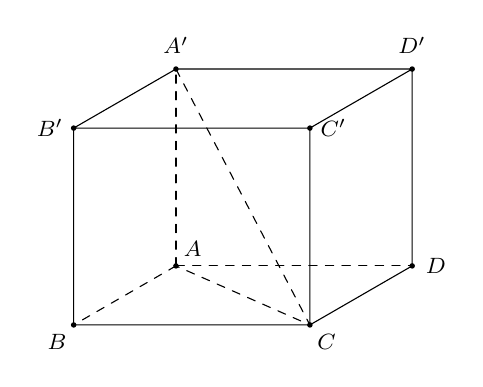
\begin{tikzpicture}[scale=1, font=\footnotesize, line join=round, line cap=round, >=stealth]
			\path
			(0,0) coordinate (A) (3,0) coordinate (D)
			(-150:1.5) coordinate (B)++(3,0) coordinate (C);
			\foreach \p in {A,B,C,D}{\path (\p)++(0,2.5) coordinate (\p');}
			\draw (B)--(C)--(C')--(B')--cycle (C)--(D)--(D')--(C') (A')--(B')--(C')--(D')--cycle;
			\draw[dashed] (A)edge(B)edge(D)edge(A') (A')--(C)--(A);
			\foreach \x/\g in {A/45, B/-135, C/-45, D/0, A'/90, B'/180, C'/0, D'/90} \fill[black] (\x) circle (1pt)+(\g:.3)node{$\x$};
		\end{tikzpicture}
	}
	\loigiai{
		Ta có $AA'\perp (ABCD)$ nên $A$ là hình chiếu của $A'$ trên $(ABCD)$.\\
		Do đó $AC$ là hình chiếu của $A'C$ trên $(ABCD)$.\\\
		Khi đó $(A'C,(ABCD))=(A'C,AC)=\widehat{A'CA}$.
	}
\end{ex}
\Closesolutionfile{ans}

\TNTF
\Opensolutionfile{ans}[ans/ansDe1-TN2]
\begin{ex}%[1D6N2-1]%[Dự án đề kiểm tra Toán 11 GHKII NH23-24- Huỳnh Xuân Tín]%[THPT Hoàng Văn Thụ- Hà Nội]
	Cho $a$, $b$, $c$ là các số thực dương và $a \neq 1$.
	\choiceTF
	{\True $\log_a b-\log_a c=\log_a \dfrac{b}{c}$}
	{$\log _{a^{\alpha}} b=\alpha \log_a b $ $(\alpha \neq 0)$}
	{$\log_a b \cdot \log_a c=\log_a(b^c)$}
	{\True $\log_a b \cdot \log_b c=\log_a c(b \neq 1)$}
	\loigiai{
		\begin{itemchoice}
			\itemch \textbf{Đúng.}\\ Ta có $\log_a b-\log_a c=\log_a \dfrac{b}{c}$.
			\itemch \textbf{Sai.}\\ Ta có $\log _{a^{\alpha}} b= \dfrac{1}{\alpha} \log_a b $ $(\alpha \neq 0)$.
			\itemch \textbf{Sai.}\\ Ta có $c \cdot \log_a b = \log_a(b^c)$.
			\itemch \textbf{Đúng.}\\ Ta có $\log_a b \cdot \log_b c=\log_a c(b \neq 1)$.
		\end{itemchoice}
	}
\end{ex}

\begin{ex}%[Chuẩn hóa M25, Nguyễn Văn Nay]%[1H8H6-1]
	\immini{Cho hình chóp $S.ABCD$ có đáy $ABCD$ là hình vuông tâm $O$ cạnh $2a$. Biết cạnh bên $SA$ vuông góc với đáy và $SA=a\sqrt{6}$.
		\choiceTF[t]
		{\True $BC \perp (SAB)$}
		{Góc giữa $BD$ và $(SAC)$ bằng $60^\circ$}
		{Hình chiếu của $SO$ lên $(ABCD)$ là $BO$}
		{\True Góc giữa đường thẳng $SO$ và mặt phẳng $(ABC)$ bằng $60^\circ$}
	}{
		\begin{tikzpicture}[>=stealth,line join=round,line cap=round,font=\footnotesize,scale=1]
			\path
			(0,0) coordinate (A) node[left]{$A$}
			(-1,-1) coordinate (B) node[left]{$B$}
			(4,0) coordinate (D) node[right]{$D$}
			($(B)+(D)-(A)$) coordinate (C) node[right]{$C$}
			(A)+(0,3) coordinate (S) node[above]{$S$}
			($(A)!.5!(C)$) coordinate (O) node[below]{$O$}
			;
			\draw (S)--(B)--(C)--(D)--cycle (S)--(C);
			\draw[dashed] (S)--(A)--(B)--(D)--(A)--(C);
			\draw[fill = gray!30] ($(A)!4pt!(S)$)--($(A)!4pt!(S)+(A)!4pt!(O)-(A)$)--($(A)!4pt!(O)$)--(A)--cycle;
			\foreach \x in {A,B,C,D,S,O} \draw[fill=black] (\x) circle (1pt);
		\end{tikzpicture}
	}
	\loigiai{
		\immini{
			\begin{itemchoice}
				\itemch \textbf{Đúng.}\\
				Ta có $\heva{&BC \perp SA\\&BC \perp AB}\Rightarrow BC \perp (SAB)$.
				\itemch \textbf{Sai.}\\
				Ta có $\heva{&BD \parallel SA\\&BD \perp AC}\Rightarrow BD \perp (SAC)$.\\
				Do đó góc giữa $BD$ và $(SAC)$ bằng $90^\circ$.
				\itemch \textbf{Sai.}\\
				Ta có $SA\perp (ABCD)$ nên hình chiếu của $SO$ lên $(ABCD)$ là $AO$.
				\itemch \textbf{Đúng.}\\
				Vì $AO$ là hình chiếu của $SO$ lên $(ABC)$ nên góc giữa $SO$ và $(ABCD)$ là góc $\widehat{SOA}$.\\
				Ta có $AC=AB\sqrt{2}=2a\sqrt{2}$.\\
				Xét tam giác $SAO$ vuông tại $A$ có
				\[\tan \widehat{SOA}=\dfrac{SA}{AO}=\dfrac{a\sqrt{6}}{a\sqrt2}=\sqrt{3}\]
				Suy ra $\widehat{SOA}=60^\circ$.
			\end{itemchoice}
		}
		{
			\begin{tikzpicture}[>=stealth,line join=round,line cap=round,font=\footnotesize,scale=1]
				\path
				(0,0) coordinate (A) node[left]{$A$}
				(-1,-1) coordinate (B) node[left]{$B$}
				(4,0) coordinate (D) node[right]{$D$}
				($(B)+(D)-(A)$) coordinate (C) node[right]{$C$}
				(A)+(0,3) coordinate (S) node[above]{$S$}
				($(A)!.5!(C)$) coordinate (O) node[below]{$O$}
				;
				\draw (S)--(B)--(C)--(D)--cycle (S)--(C);
				\draw[dashed] (S)--(A)--(B)--(D)--(A)--(C) (S)--(O);
				\draw[fill = gray!30] ($(A)!4pt!(S)$)--($(A)!4pt!(S)+(A)!4pt!(O)-(A)$)--($(A)!4pt!(O)$)--(A)--cycle;

				\foreach \x in {A,B,C,D,S,O} \draw[fill=black] (\x) circle (1pt);
			\end{tikzpicture}
		}
	}
\end{ex}
\Closesolutionfile{ans}

\TNSA
\Opensolutionfile{ans}[ans/ansDe1-TN3]
\begin{ex}%[1D6N3-2]%[Dự án đề kiểm tra Toán 11 CHKII NH23-24- Ngô Tất Thành]%[THPT Phạm Văn Sáng - Tp HCM]
	Hàm số $y=\log_2 (1-x^2)$ có tập xác định là $(a;b)$. Tính $S=a^2+b^2$.
	\shortans{$S=2$}
	\loigiai{
		Điều kiện xác định của hàm số $y=\log_2 (1-x^2)$ là $1-x^2>0 \Leftrightarrow -1<x<1$.\\
		Vậy tập xác định của hàm số là $\mathscr{D}=(-1;1)$. Nên $a=-1$, $b=1$.\\
		Suy ra $S=a^2+b^2=2$.
	}
\end{ex}

\begin{ex}%[1D6H4-5]%[Tex hoá đề CK2-form 2025-Đợt 2-Nguyễn Kiều Nhã Tú]
	Bất phương trình $\log_2^2 (2x)-4\log_2 4x+4<0$ có số nghiệm nguyên tương ứng là
	\shortans{$7$}
	\loigiai{
		Điều kiện $x>0$, khi đó
		\allowdisplaybreaks
		\begin{eqnarray*}
			&&\log_2^2 (2x)-4\log_2 4x+4<0\\
			&\Leftrightarrow& \log_2^2 (2x)-4\left(1+\log_2 2x\right)+4<0\\
			&\Leftrightarrow& \log_2^2 (2x)-4\log_2 2x<0\\
			&\Leftrightarrow& 0<\log_2 2x<4\\
			&\Leftrightarrow& 1<2x<16\\
			&\Leftrightarrow& \dfrac{1}{2}<x<8.
		\end{eqnarray*}
		Đối chiếu với điều kiện, ta có số nghiệm nguyên của phương trình là $7$.}
\end{ex}

\begin{ex}%[1D6V3-5]
	Một người lập kế hoạnh gửi tiết kiệm ngân hàng như sau: Đầu tháng 1 năm 2023, người đó gửi 10 triệu đồng; sau mỗi đầu tháng tiếp theo, người đó gửi số tiền nhiều hơn $10\%$ so với số tiền đã gửi ở tháng liền trước đó. Biết rằng lãi suất ngân hàng không đổi là $0{,}5\%$ mỗi tháng và được tính theo hình thức lãi kép. Với kế hoạnh như vậy, đến hết tháng 12 năm 2024, số tiền của người đó trong tài khoản tiết kiệm là bao nhiêu triệu đồng?
	\shortans{$922$}
	\loigiai{
	Với $A=10$ triệu, $a=0{,}1$, $r=0{,}005$.\\
	Đầu tháng 2: $A(1+r)+A(1+a)$.\\
	Đầu tháng 3: $A(1+r)^2+A(1+a)(1+r)+A(1+a)^2$.\\
	Đầu tháng 4: $A(1+r)^3+A(1+a)(1+r)^2+A(1+a)^2(1+r)+A(1+a)^3$.\\
	….\\
	Đầu tháng $n$: $A\left[(1+r)^{n-1}+(1+r)^{n-2}(1+a)+\cdots +(1+r)(1+a)^{n-2}+(1+a)^{n-1}\right]$.\\
	Hết tháng $n$: $A\left[(1+r)^{n-1}+(1+r)^{n-2}(1+a)+\cdots +(1+r)(1+a)^{n-2}+(1+a)^{n-1}\right](1+r)$.\\
	Gọi $B$ là số tiền của người đó trong tài khoản tiết kiệm đến hết tháng 12 năm 2024.
	Khi đó $n=24$.\\
	Ta có $B=A\cdot\dfrac{(1+a)^n-(1+r)^n}{a-r}(1+r)\approx 922{,}7$.}
\end{ex}

\begin{ex}%[1H8V6-2]
	Một chân cột bằng gang có dạng hình chóp cụt tứ giác đều có cạnh đáy lớn bằng $2a$, cạnh đáy nhỏ bằng $a$, chiều cao $h = 2a$ và bán kính đáy phần trụ rỗng bên trong bằng $\dfrac{a}{2}$. Tìm góc phẳng nhị diện tạo bởi mặt bên và mặt đáy (đơn vị tính góc là độ, làm tròn đến hàng đơn vị độ).

	\shortans{$76$}
	\loigiai
	{
		Gọi hình chóp cụt tứ giác đều là $ABCD.A'B'C'D'$ với $CD = 2a$, $C'D' = a$.
		\begin{center}
			\begin{tikzpicture}[>=stealth,line join=round,line cap=round,font=\footnotesize,scale=1]
				\coordinate[label=above left:{$A$}] (A) at (0,0);
				\coordinate[label=below left:{$B$}] (B) at (-2,-1.75);
				\coordinate[label=below right:{$C$}] (C) at (3.5,-1.75);
				\coordinate[label=right:{$D$}] (D) at ($(A)+(C)-(B)$);
				\coordinate[label=below:{$O$}] (O) at (intersection of A--C and B--D);
				\coordinate (S) at ($(O)+ (0,4)$);
				\coordinate[label=above left:{$A'$}] (A') at ($(S)!0.3!(A)$);
				\coordinate[label=above left:{$B'$}] (B') at ($(S)!0.3!(B)$);
				\coordinate[label=below left:{$C'$}] (C') at ($(S)!0.3!(C)$);
				\coordinate[label=above right:{$D'$}] (D') at ($(S)!0.3!(D)$);
				\coordinate[label=left:{$O'$}] (O') at ($(S)!0.3!(O)$);
				\coordinate[label=below right:{$M$}] (M) at ($(C)!0.5!(D)$);
				\coordinate[label=right:{$N$}] (N) at ($(C')!0.5!(D')$);
				%\pic["$45^\circ$"{shift={(1pt,-3pt)}},draw,angle radius=4mm,angle eccentricity=1.79] {angle = N--M--O};
				\draw pic[draw,angle radius=2mm] {right angle = O'--O--M};
				\path
				($(O)!(N)!(M)$)coordinate [label=below:{$H$}](H);
				\draw pic[draw,angle radius=2mm] {right angle = N--H--M};
				\draw
				(B)--(C)--(D)
				(A')--(B')--(C')--(D') --cycle
				(B)--(B') (C)--(C') (D)--(D')
				(M)--(N)
				;
				\draw[dashed] (A')--(A) (B)--(A)--(D) (M)--(O)--(O')--(N) (N)--(H);
				\foreach \p in {A,B,C,D,O,M,N,O',H,B',C',A'}
				\fill (\p) circle (1.2pt);
			\end{tikzpicture}
		\end{center}
		Gọi $O$,$O'$ lần lượt là tâm hai đáy của hình chóp cụt tứ giác đều $ABCD.A'B'C'D'$. Suy ra $OO' = 2a$.\\
		Gọi $M$, $N$ lần lượt là trung điểm $CD$, $C'D'$.\\ Ta có $MN \perp CD$, $OM \perp CD$.\\
		Gọi $H$ là hình chiếu của $N$ trên $OM$.\\
		Bán kính đáy trụ rỗng bên trong là $ON = \dfrac{a}{2}$.\\
		Ta có $OM = \dfrac{AD}{2} = a$. Suy ra $HM = OM - OH = \dfrac{a}{2}$.\\
		Khi đó góc nhị diện $[N, CD, H]$ là $\widehat{NMH}$.\\
		Trong $\triangle HMN$ vuông tại $H$ với $NH = h = 2a$, $HM = \dfrac{a}{2}$ ta có
		\[\tan \widehat{NMH} = \dfrac{NH}{HM} = \dfrac{2a}{\dfrac{a}{2}} = 4.\]
		Suy ra $\widehat{NMH} = 75^\circ 57' 49{,}52'\approx 76^\circ$.
	}
\end{ex}

\Closesolutionfile{ans}

\TL
\begin{ex}%[1D6H4-4]
	Giải phương trình $\log _{\frac{1}{5}}\left(x^2-6 x+18\right)+2 \log _5(x-4)=0$.
	\loigiai{
		Điều kiện xác định $\heva{&x^2-6 x+18>0\\&x-4>0}\Leftrightarrow x>4$.\\
		Khi đó
		\begin{eqnarray*}
			&&\log _{\frac{1}{5}}\left(x^2-6 x+18\right)+2 \log _5(x-4)=0\\
			&\Leftrightarrow& \log_5 (x-4)^2=\log_5 \left(x^2-6 x+18\right)\\
			&\Leftrightarrow& x^2-8x+16=x^2-6 x+18\\
			&\Leftrightarrow& x=-1.~ \text{(loại)}
		\end{eqnarray*}
		Vậy phương trình vô nghiệm.
	}
\end{ex}

\begin{ex}%[1D6H4-6]
	Nếu khối lượng carbon-14 trong cơ thể sinh vật lúc chết là $M_0(\mathrm{~g})$ thì khối lượng carbon-14 còn lại (tính theo gam) sau $t$ năm được tính theo công thức $M(t)=M_0\left(\frac{1}{2}\right)^{\frac{t}{T}}(\mathrm{~g})$, trong đó $T=5730$ (năm) là chu kì bán rã của carbon-14. Nghiên cứu hoá thạch của một sinh vật, người ta xác định được khối lượng carbon-14 hiện có trong hoá thạch là $5 \cdot 10^{-13} \mathrm{~g}$. Nhờ biết tỉ lệ khối lượng của carbon- 14 so với carbon- 12 trong cơ thể sinh vật sống, người ta xác định được khối lượng carbon-14 trong cơ thể lúc sinh vật chết là $M_0=1,2 \cdot 10^{-12}(\mathrm{~g})$. Sinh vật này sống cách đây bao nhiêu năm? (Làm tròn kết quả đến hàng trăm.)
	% \shortans[0]{7200}
	\loigiai{
		Gọi $t$ là thời gian từ lúc sinh vật chết đến nay. Ta có
		\[
			\begin{aligned}
				5 \cdot 10^{-13}=1,2 \cdot 10^{-12} \cdot\left(\frac{1}{2}\right)^{\frac{t}{T}} & \Leftrightarrow\left(\frac{1}{2}\right)^{\frac{t}{T}}=\frac{5}{12} \Leftrightarrow \frac{t}{T}=\log _{\frac{1}{2}} \frac{5}{12} \\
				                                                                                & \Leftrightarrow t=T \log _{\frac{1}{2}} \frac{5}{12}=-5\,730 \cdot \log _2 \frac{5}{12} \approx 7\,237 \approx 7\,200
			\end{aligned}
		\]
		Vậy sinh vật này sống cách đây khoảng $7\,200$ năm.
	}
\end{ex}

\begin{ex}%[1H8V2-3]
	Cho hình chóp tứ giác $ S. ABCD$ có đáy là hình vuông cạnh $a$. Mặt bên $SAD$ là tam giác đều và ở trong mặt phẳng vuông góc với đáy. Gọi $M$, $N$, $P$ lần lượt là trung điểm $SB$, $BC$, $CD$. Chứng minh $AM\perp BP$.
	\loigiai{
	\begin{center}
		% Đại học khối A năm 2007
		\begin{tikzpicture}[scale=0.8, font=\footnotesize, line join=round, line cap=round, >=stealth]
			\path
			(0,0) coordinate (A)
			($(A)+(5,0)$) coordinate (B)
			($(A)+(-2,-2)$) coordinate (D)
			;
			\coordinate (C) at ($(B)+(D)-(A)$);
			\coordinate (H) at ($(A)!0.5!(D)$);
			\coordinate (S) at ($(H)+(0,5)$);
			\coordinate (M) at ($(S)!0.5!(B)$);
			\coordinate (N) at ($(B)!0.5!(C)$);
			\coordinate (P) at ($(C)!0.5!(D)$);
			\path
			(intersection of H--C and P--B) coordinate (I)
			(intersection of A--N and P--B) coordinate (G)
			pic [draw, angle radius = 2.5mm]{right angle = A--H--S}
			pic [draw, angle radius = 2.5mm]{right angle = P--I--C}
			pic [draw, angle radius = 2.5mm]{right angle = P--G--N}
			;
			\draw (S) -- (B) -- (C) -- (D) -- (S) --(C) -- (M) -- (N);
			\draw[dashed] (B) -- (A) -- (S) (A) -- (D) (S) -- (H) (P) -- (B) (A) -- (N) (H) -- (C) (P) -- (M) -- (A);
			\foreach \x/\g in {A/180,B/0,C/0,D/180,M/45,N/-20,P/-90,H/180,S/90} \fill[black](\x) circle (1pt)+(\g:3mm) node{$\x$};

		\end{tikzpicture}
		\begin{tikzpicture}[scale=0.7, font=\footnotesize, line join=round, line cap=round, >=stealth]
			\def \canh{5}
			\path
			(0,0) coordinate (A)
			(\canh,0) coordinate (B)
			(0,-\canh) coordinate (D)
			($(B)+(D)-(A)$) coordinate (C)
			($(A)!0.5!(D)$) coordinate (H)
			($(B)!0.5!(C)$) coordinate (N)
			($(C)!0.5!(D)$) coordinate (P)
			(intersection of H--C and P--B) coordinate (I)
			(intersection of A--N and P--B) coordinate (G)
			pic [draw, angle radius = 2.5mm]{right angle = P--I--C}
			pic [draw, angle radius = 2.5mm]{right angle = P--G--N}
			pic [draw, angle radius = 3.5mm]{angle = P--B--C}
			pic [draw, angle radius = 4.5mm]{angle = H--C--D}
			;
			\draw ($(C)+(165:0.9)$) node {$1$};
			\draw ($(B)+(-105:0.9)$) node {$1$};
			\draw (A) -- (B) -- (C) -- (D) -- (A) -- (N) (B) -- (P) (H) -- (C);
			\foreach \x/\g in {A/90,B/90,C/-90,D/-90,H/180,N/0} \fill[black](\x) circle (1pt)+(\g:3mm) node{$\x$};

		\end{tikzpicture}
	\end{center}
	Hạ $SH\perp AD$ tại $H$.\\
	Vì $SAD$ là tam giác đều nên $SH=\dfrac{a\sqrt{3}}{2}$.\\
	Vì mặt phẳng $\left(SAD\right)$ vuông góc mặt phẳng $\left(ABCD\right)$ nên có $AD$ là giao tuyến.\\
	Suy ra $SH\perp (ABCD)$.\\
	Ta có $AN\parallel HC$ và $MN\parallel SC$.\\
	Mà $AM,MN\subset (AMN)$ và $HC,SC\subset \left(SHC\right)$.\\
	Suy ra mặt phẳng $\left(AMN\right)$ song song mặt phẳng $\left(SHC\right)$.\\
	Trong hình vuông $ABCD$ ta có $\triangle BCP=\triangle CDH$ (c.g.c) nên $\widehat{B_1}=\widehat{C_1}$.\\
	Mà $\widehat{B_1}+\widehat{P_1}=90^{\circ}\Rightarrow \widehat{C_1}+\widehat{P_1}=90^{\circ}\Rightarrow CH\perp PB$.\\
	Ta có $\heva{& BP\perp CH \\& BP\perp SH}\Rightarrow BP\perp \left(SHC\right)\Rightarrow BP\perp \left(AMN\right)\Rightarrow BP\perp AM$.
	}
\end{ex}

% \Closesolutionfile{ansbook}
% \HetDe
% \label{De1}
% %
% \cleardoublepage
% \setcounter{page}{1}
% \rfoot{Trang \thepage/\pageref{DA1} - Đáp án trắc nghiệm Mã đề 1}
% \begin{center}
% 	\bfseries ĐÁP ÁN TRẮC NGHIỆM MÃ ĐỀ 1
% \end{center}

% \inputansbox{10}{ans/ansDe1-TN1}
% \inputansbox[3]{2}{ans/ansDe1-TN2}
% \inputansbox{3}{ans/ansDe1-TN3}
% \label{DA1}
%
